\documentclass[12pt]{article}
\usepackage{amssymb}
\usepackage{amsmath}
\usepackage{color}
\usepackage{tikz}
\usetikzlibrary{cd}
\tikzcdset{
	arrow style=tikz,
	diagrams={>={Straight Barb[scale=0.8]}}
}

\newcommand{\dslash}{/\hspace{-2.5pt}/}

\begin{document}

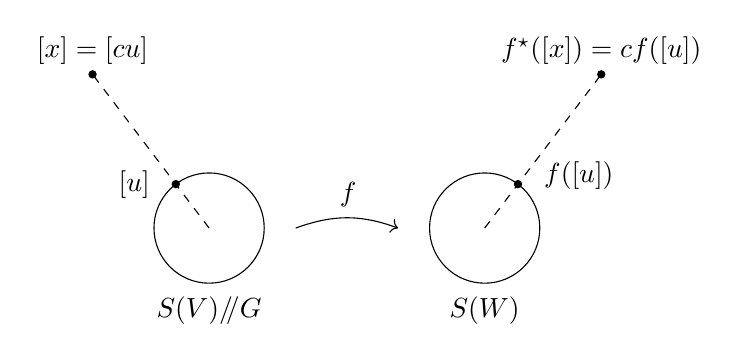
\begin{tikzpicture}
\coordinate (u) at (-0.6042*0.7,0.79682*0.7);
\coordinate (x) at (-3.5*0.6042*0.7,3.5*0.7968*0.7);
\draw[dashed] (0,0) -- (x);
\draw[fill=none] (0,0) circle (1.0*0.7) node [yshift=-30] {$S(V)\dslash G$};
\draw[fill] (u) circle (1.3 pt) node [xshift=-15] {$[u]$};
\draw[fill] (x) circle (1.3 pt) node [above] {$[x]=[cu]$};
\draw [->] (1.1,0) to [out=20,in=160] (2.4,0) node[xshift=-18,yshift=12] {$f$};
\coordinate (gu) at (3.5+0.6042*0.7,0.79682*0.7);
\coordinate (gx) at (3.5+3.5*0.6042*0.7,3.5*0.7968*0.7);
\draw[dashed] (3.5,0) -- (gx);
\draw[fill=none] (3.5,0) circle (1.0*0.7) node [yshift=-30] {$S(W)$};
\draw[fill] (gu) circle (1.3 pt) node [xshift=22,yshift=3] {$f([u])$};
\draw[fill] (gx) circle (1.3 pt) node [above] {$f^\star([x])=cf([u])$};
\end{tikzpicture}

\end{document}